% !TEX root = tesis.tex
\pagestyle{fancy}
\chapter{Mirando al Sol invisible}
\chaptermark{El Sol invisible}
\label{chap:uno}

Nuestra especie, por medio de sus sentidos, es consciente del mundo a su alrededor, no obstante ha invertido miles de años en tratar de entender aquello que con los sentidos podemos percibir, usando la razón. Comprender el espacio en el que habitamos y las complejas relaciones entre sus diversos elementos representa una de las más altas aspiraciones de la raza humana.

Así, con nuestros ojos vemos a través de la luz sin poder entender completamente su naturaleza y origen. Hoy nuestra compresión del fenómeno es ligeramente superior, no solo gracias al desarrollo de complejos modelos teóricos, sino a la construcción de instrumentos que nos permiten observar más allá de nuestros sentidos.

La edad del Universo se ha podido estimar en \num{13.787(20)e9} años a partir de mediciones precisas de la radiación de fondo de microondas (CMB) por parte de satélites y modelos cosmológicos \cite{plank18}. No obstante, nuestra compresión de lo ocurrido el instante del \emph{big bang}, hasta aproximadamente \SI{e-43}{\second} después de él, resulta inaccesible para las leyes de la Física. Podemos suponer que en el principio el Universo era infinitamente pequeño y caliente; lo cual implica que las \num{4} interacciones fundamentales estaban unificadas. A medida que el Universo se expande, la temperatura también disminuye; trayendo consigo la separación de interacciones fundamentales (gravedad e interacciones nuclear fuerte y electrodébil), además de una serie de fenómenos que aún no entendemos del todo. Uno de estos procesos es la de inflación cósmica (expansión acelerada), la cual podría explicar la estructura homogénea del Universo a gran escala. Por otro lado está el proceso de bariogénesis. De éste se desconoce su mecanismo, pero se supone estuvo presente en las etapas iniciales del Universo y dio origen a la asimetría entre la cantidad de materia y antimateria.

A partir de lo \SI{e-10}{\second} después del \emph{big bang} nuestra compresión de los fenómenos físicos es más clara debido a que la temperatura del Universo se encuentra en la región de energía explorada usando el LHC y descrita con precisión a través del \emph{modelo estándar}. En esta etapa la temperatura del Universo aún era demasiado alta para permitir la formación de hadrones, por lo que la materia se encuentra en una fase de plasma quark-gluones. Aproximadamente a los \SI{e-6}{\second} el Universo se enfría lo suficiente para que quarks y gluones se unan para formar protones, neutrones y demás hadrones. A un segundo desde el inicio de la expansión la temperatura es cercana a los \SI{e10}{\kelvin}; el Universo se compone principalmente de fotones, electrones y neutrinos; además de algunos protones y neutrones. Cuando la temperatura cae alrededor de los \SI{e9}{\kelvin} (\SI{100}{\second}), neutrones y protones no tienen suficiente energía para escapar a la atracción de la fuerza nuclear fuerte y se combinan para formar los primeros átomos de \ce{^{2}H}, \ce{^{4}He}, \ce{Li} y \ce{Be}. Durante esta época el plasma que constituye el universo es opaco a los fotones, ya que los electrones libres interaccionan mediante dispersión de Thomson con los fotones; dejándoles a éstos un camino libre medio muy corto.

Un punto de inflexión ocurre cuando el Universo tiene una edad de \num{3.8e5} años. Aquí el enfriamiento del plasma permite que la atracción electromagnética una electrones y protones para formar los primeros átomos neutros. En este instante se vuelve posible que los fotones viajen largas distancias sin ser absorbidos. Son estos fotones, corridos hacia el rojo, los que constituyen la radiación de fondo de microondas (CMB) y que brindan una las principales pruebas del modelo del \emph{big bang}.

Tendrían que transcurrir algunos millones de años más para que las primeras galaxias se comenzarán a formar. Esto ocurrió en zonas donde existía una ligera mayor concentración de materia, las cuales fueron frenadas de su expansión por la atracción gravitacional. A medida que el gas en estas regiones colapsaba, los átomos dentro de ellas colisionaban incrementando su energía cinética. La edad oscura del Universo\footnote{Llamada así por la falta de un mecanismo para producir fotones.} llegaría a su fin a medida que los efectos gravitatorios y las colisiones fueron calentando el material y produciendo reacciones nucleares hasta que se formaron las estrellas.

Es así como la formación del Sol representa tan solo un pequeño instante en la historia del Universo. Nuestro interés por él surge más bien de su estrecha relación con la vida de nuestra especie en la Tierra. A pesar de esto, no debemos subestimar su importancia en el desarrollo de la Astronomía y Astrofísica. Es a través del estudio conjunto del Universo lejano y de los procesos que ocurren en el Sol que nuestro entendimiento de lo que nos rodea se ha enriquecido. Si además abordamos este estudio desde la perspectiva de la Física de partículas, mirar al Sol invisible nos presenta un laboratorio único para estudiar fenómenos extraordinariamente complejos.

\section{Estructura interna del Sol}

El Sol es una estrella joven de unos \num{4.5e9} años de segunda generación, lo cual implica que contiene materia más pesada que expulsada de la generación previa de estrellas cuando éstas se convirtieron en supernovas. Su volumen es de \SI{1.41d27}{\cubic\metre} y tiene temperatura superficial de \SI{5780}{\kelvin}. El Sol es el objeto más grande de nuestro sistema planetario; una (casi) esfera de plasma compuesta en un \SI{92.1}{\percent} de Hidrógeno, \SI{7.8}{\percent} Helio y \SI{0.1}{\percent} de otros materiales más pesados.

Los fotones que nos permiten ver el mundo que nos rodea tienen su origen en el núcleo solar mediante fusión nuclear. El núcleo ocupa la distancia desde el centro hasta \num{0.25} del radio solar ($R_{s}$) \cite{fisica13}. En él se encuentra el \SI{50}{\percent} de la masa del Sol, con una densidad de \SI{1.5d5}{\kilogram\per\cubic\metre}. Aun cuando no podemos ver en el interior del Sol, existen modelos generalmente aceptados de cómo está constituido y cuáles son los procesos que transportan la energía generada en su interior hasta su atmósfera. En el núcleo la temperatura (\SI{1.5d7}{\kelvin}) y presión (\SI{2.6e17}{\pascal}) son tan altas que las interacciones nucleares se dan de forma espontánea y dado que el Hidrógeno es el elemento más abundante, las reacciones protón-protón ($p^{+}-p^{+}$) para crear Helio son las más abundantes. Cerca de \num{3.6d38} protones por segundo son convertidos en núcleos de Helio, lo que equivale a una tasa de producción de energía de \SI{3.8e26}{\watt} \cite{lang09}.

Las reacciones $p^{+}-p^{+}$ se desarrollan en tres etapas:

\begin{enumerate}
  \item Producción de deuterón: $p^{+}+p^{+}\rightarrow\ce{^{2}H^{+}}+e^{+}+\nu_{e}$.
  \item Fusión de deuterón para producir Helio: $\ce{^{2}H^{+}}+p^{+}\rightarrow\ce{^{3}He}+\gamma$.
  \item Finalmente generación de $\ce{^{4}He}$ , para lo cual existen varias reacciones, sin embargo la más probable es: $\ce{^{3}He}+\ce{^{3}He}\rightarrow\ce{^{4}He}+2p^{+}$.
\end{enumerate}

En estrellas del tamaño de nuestro Sol la última reacción es el principal mecanismo de producción de $He$ y ocurre en \SI{\approx 84}{\percent} de los casos \cite{adelberger11}. El resultado neto del ciclo protón-protón es la conversión de \num{6} protones en \ce{^{4}He} con la liberación de \SI{26.73}{\mega\electronvolt}. Los neutrinos emitidos en la fusión toman un promedio de \SI{0.25}{\mega\electronvolt} de energía cada uno; y de esta forma cada átomo de \ce{H} en el proceso lleva a la emisión de \SI{6.55}{\mega\electronvolt} de energía electromagnética \cite{noyes82}.

Otro reacción importante en la que se convierte hidrógeno en helio es el \emph{ciclo CNO} (carbono-nitrógeno-oxigeno). En el Sol sólo \SI{10}{\percent} del total de reacciones nucleares son ciclo CNO, sin embargo en estrellas más masivas esta es la fuente de energía principal.

Las principales reacciones que componen el ciclo CNO se describen a continuación:

\begin{enumerate}
	\item $\ce{_{6}^{12}C}+p^{+}\rightarrow\ce{_{7}^{13}N}+\gamma+\SI{1.9}{\mega\electronvolt}$.
	\item $\ce{_{7}^{13}N}\rightarrow\ce{_{6}^{13}C}+e^{+}+\nu_{e}+\SI{1.2}{\mega\electronvolt}$.
	\item $\ce{_{6}^{13}C}+p^{+}\rightarrow\ce{_{7}^{14}N}+\gamma+\SI{7.5}{\mega\electronvolt}$.
	\item $\ce{_{7}^{14}N}+p^{+}\rightarrow\ce{_{8}^{15}O}+\gamma+\SI{7.3}{\mega\electronvolt}$.
	\item $\ce{_{8}^{15}O}\rightarrow\ce{_{7}^{15}N}+e^{+}+\nu_{e}+\SI{1.7}{\mega\electronvolt}$.
	\item $\ce{_{7}^{15}N}+p^{+}\rightarrow\ce{_{6}^{12}C}+\ce{_{2}^{4}He}$.
\end{enumerate}

Al finalizar el ciclo, el núcleo de $C$ con el que se inicia el ciclo se regenera y por lo tanto éste actúa como un catalizador \cite{golub14}.

A medida que disminuye presión y temperatura, la fusión nuclear no puede llevarse a cabo, con lo cual se considera termina el núcleo. Sólo los rayos $\gamma$ producto de las reacciones pueden transportar la energía generada en el núcleo hacia las capas superiores del Sol. Sin embargo, debido a la alta densidad del medio, éstos no pueden recorrer una gran distancia sin colisionar con el plasma del medio y perder energía. Colisión tras colisión los fotones son dispersados y parte de su energía es convertida en fotones menos energéticos cuya longitud de onda hacia el rango de los rayos $X$. Con mucha dificultad un fotón tarda \num{\approx 1e6} años en atravesar una distancia de $\num{0.5}R_{s}$ \cite{fisica13}. A esta región entre \num{0.25} y $\num{0.7}R_{s}$, en donde sólo los fotones transportan energía, se le denomina \emph{zona de radiación}.

Después de los $\num{0.7}R_{s}$, la presión y temperatura en el Sol han disminuido considerablemente y puede formase hidrógeno molecular $H_{2}$, el cual es capaz de absorber grandes cantidades de radiación ultravioleta. Debido a esto, el transporte de energía deja de hacerse por medio de radiación. El gradiente de temperatura entre la parte superior y la parte más baja hace que el plasma caliente suba y el frío baje, formando corrientes de convección. Estos movimientos forman celdas convectivas de diferentes tamaños, que al ser observadas mediante telescopios de alta resolución, se muestran como gránulos en la superficie solar cuyo centro es más brillante que las orillas. Las áreas más brillantes indican la presencia de material caliente en ascenso. La zona en donde se lleva a cabo este proceso se conoce como \emph{zona convectiva} y tiene una profundidad que va desde \num{0.7} hasta $\num{1.0}R_{s}$.

La \emph{atmósfera solar} es la parte del Sol que se encuentra al exterior de la zona convectiva y donde la energía del núcleo escapa hacia el espacio principalmente en forma de radiación. Es la parte visible del Sol y consta de tres capas: \emph{fotosfera}, \emph{cromosfera} y \emph{corona}. La fotosfera es una capa delgada, con una temperatura cercana a los \SI{5700}{\kelvin} \cite{noyes82}. Una característica sobresaliente de la fotosfera son las \emph{manchas solares}; regiones oscuras que tienen diámetros que van desde \num{e3} hasta \SI{e5}{\kilo\metre}. Las manchas son la manifestación visible de las cuerdas de flujo magnético que emergen de la zona convectiva hacia la atmósfera superior (una explicación más detallada se da en la siguiente sección). La magnitud del campo magnético en las manchas es tan grande que dificulta la circulación del plasma en su interior, lo cual logra aislarlo de su entorno y generar diferencias de temperatura (entre \num{1000} y \SI{2000}{\kelvin} más frías que la fotosfera \cite{fisica13}). Es debido a esta temperatura inferior que el material dentro de la mancha radia una menor cantidad de fotones, lo que desde nuestra perspectiva se ve como regiones oscuras.

El número de manchas es variable y está estrechamente relacionado con el ciclo de actividad solar, cuya duración es de aproximadamente \num{11} años. Las manchas aparecen abruptamente al inicio del ciclo solar. Su número aumenta conforme la forma del campo se aleja de la forma dipolar y alcanza un máximo cuando al campo alcanza la forma toroidal. Las primeras manchas del ciclo aparecen en latitudes cercanas a  $\ang{30}\mathbf{N}$ y $\ang{30}\mathbf{S}$ \cite{golub14}. Al pasar el tiempo, estas manchas desaparecen y surgen nuevas, cada vez más cerca del ecuador solar. A la migración de las manchas solares durante el ciclo se le conoce como \emph{ley de Spörer} \cite{noyes82}.

En la región superior de la fotosfera la temperatura alcanza un valor mínimo de \SI{4400}{\kelvin}. Contrario a lo que se supondría, al alejarnos de la superficie solar, en la cromosfera (entre \num{1000} y \SI{2000}{\kilo\metre} de altura), la temperatura crece lentamente hasta los \SI{6000}{\kelvin}. Al llegar a los \SI{2300}{\kilo\metre}, ésta alcanza \SI{1d6}{\kelvin}. Ambos fenómenos han sido estudiados ampliamente, sin embargo su mecanismo no es totalmente entendido. La \emph{zona de transición}, la región donde se presenta el cambio brusco de temperatura, marca el límite entre la cromosfera y la corona. Debido a las altas temperaturas en la región, el gas en la corona no puede ser retenido por la atracción gravitacional del Sol y en consecuencia se extiende por todo el medio interplanetario. La expansión del gas coronal no puede realizarse con velocidad igual a cero ya que esto implica que la presión del fluido permanece finita a distancias infinitas del Sol. En consecuencia, la única solución posible es que la velocidad incremente y por lo tanto disminuya la presión a medida que nos alejamos del Sol. A medida que la velocidad va en aumento el flujo se vuelve supersónico y recibe el nombre de \emph{viento solar}.

\section{Ráfagas solares}

Las ráfagas solares (también conocidas como fulguraciones) son fenómenos explosivos que se observan en la atmósfera del Sol, la cual está llena de plasma magnetizado. La energía que se libera durante una ráfaga se encuentra en el rango de \SI{e21}{\joule} a \SI{e25}{\joule} y puede emitirse en diferentes productos. La magnitud espacial de las cuerdas magnéticas de la ráfaga va desde los \SI{e3}{\metre} hasta los \SI{e5}{\metre}, aunque varia de evento a evento. El tamaño afecta directamente la duración (entre \SI{e3}{\second} y \SI{e4}{\second}) y la cantidad de energía liberada.

Las ráfagas se observan en un amplio rango del espectro electromagnético; en ondas de radio, radiación óptica, rayos X y rayos $\gamma$. La figura \ref{fig:flare-euv} muestra un ejemplo de la observación una ráfaga por medio del satélite SDO (Solar dynamics observatory), ocurrida el \num{19} de Julio de \num{2012} (la explicación detallada de la imagen se da más adelante). Por otro lado, las explosiones puede acelerar iones y electrones a energías relativistas; que a su vez pueden producir otras partículas. De forma cualitativa podemos clasificar e las fulguraciones en cinco grupos de acuerdo a la intensidad de la emisión de rayos X, la cual es indicativa de la cantidad de energía que radia el plasma coronal. Para la clasificación de grupos se usa la banda de \SI{0.1}{\nano\metre} a \SI{0.8}{\nano\metre} del satélite GOES, localizado a una distancia de \SI{1}{AU}. La clasificación es la siguiente: \textbf{A}(\SI{\geq e-8}{\watt\per\square\metre}), \textbf{B}(\SI{\geq e-7}{\watt\per\square\metre}), \textbf{C}(\SI{\geq e-6}{\watt\per\square\metre}), \textbf{M}(\SI{\geq e-5}{\watt\per\square\metre}) y \textbf{X}(\SI{\geq e-4}{\watt\per\square\metre}).

La enorme cantidad de energía liberada durante la explosión puede explicarse a través de los modelos de reconexión magnética, propuestos originalmente entre \num{1946} y \num{1958} \cite{giovanelli,hoyle,sweet,parker}. En estos modelos, cuerdas de flujo magnético (tubos de flujo torcidos) emergen a la superficie solar debido al efecto de boyancia originado por las diferencias de densidad entre el plasma del tubo y su alrededor. Una vez que las cuerdas se encuentran en la superficie, su campo magnético es comprimido por el plasma en su vecindad que se mueve a una cierta velocidad. El resultado de la compresión crea zonas en donde interaccionan líneas de campo de polaridad opuesta y en la región neutra surge una hoja de corriente. Eventualmente el flujo de corriente produce un gradiente del campo magnético y la topología se reorganiza para encontrar una configuración de menor energía \cite{shiba11}. A través de este proceso, la energía magnética almacenada en la hoja de corriente se convierte en energía cinética y térmica; además de estar acompañada de intensos campos eléctricos los cuales pueden ser los responsables de la aceleración de partículas.

La existencia del proceso de reconexión magnética fue comprobada mediante observaciones en rayos X del satélite Yokoh \cite{masuda,tsuneta} y simulaciones magnetohidrodinámicas (MHD) de la atmósfera solar  \cite{yokoyama}; sin embargo se necesitan observaciones más detalladas para confirmar los modelos. Otro avance importante hacia el establecimiento de los modelos de reconexión se dio en Julio de \num{2012}, con la observación por parte del satélite SDO de la formación de cuerdas magnéticas. La figura \ref{fig:flare-euv} muestra la evolución temporal de una ráfaga ocurrida el dia \num{19}. En el panel superior izquierdo se observa el lapso de tiempo antes de la explosión, a una longitud de onda de \SI{17}{\nano\metre}, la cual sirve para estudiar la corona solar en estado de reposo. El panel superior derecho muestra el mismo evento minutos después; en la parte derecha de la imagen se aprecia una zona que se ilumina ligeramente naranja (marcada con un circulo rojo). La intensa emisión en tres bandas de UVE (de \num{10} a \SI{120}{\nano\metre}) está asociada con los campos magnéticos de la cuerda. Los paneles inferiores fueron registrados \SI{8}{\hour} después, cuando la compleja estructura del campo magnético se reorganiza dando lugar a la ráfaga.

\begin{figure}
        \centering
        \begin{subfigure}[b]{0.49\textwidth}
                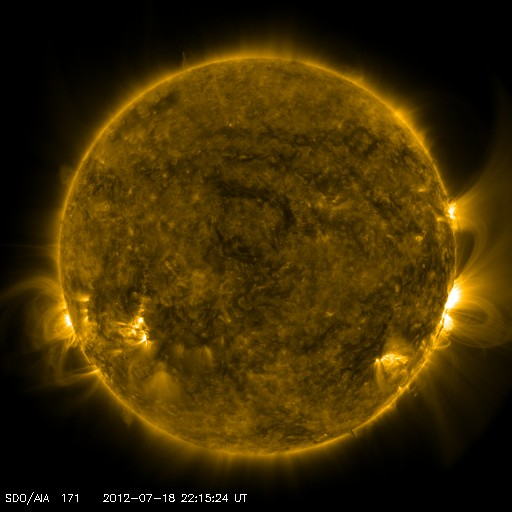
\includegraphics[width=7.25cm]{sdo120718-2215-17}
                \caption*{Imagen en la banda de \SI{17}{\nano\metre}.}
        \end{subfigure}
        \begin{subfigure}[b]{0.49\textwidth}
                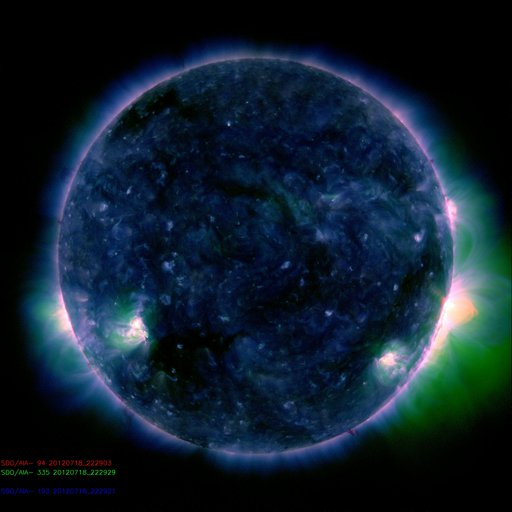
\includegraphics[width=7.25cm]{sdo120718-2229-c}
                \caption*{Imagen compuesta: \SI{9}{\nano\metre}, \SI{19}{\nano\metre} y \SI{33}{\nano\metre}.}
        \end{subfigure}
        \begin{subfigure}[b]{0.49\textwidth}
                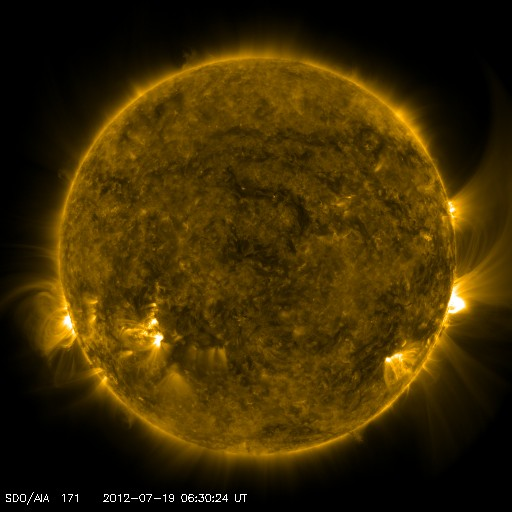
\includegraphics[width=7.25cm]{sdo120719-0630-17}
                \caption*{Imagen en la banda de \SI{17}{\nano\metre}.}
        \end{subfigure}
        \begin{subfigure}[b]{0.49\textwidth}
                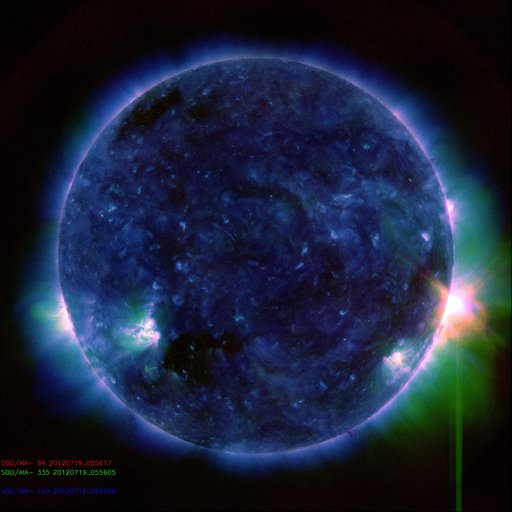
\includegraphics[width=7.25cm]{sdo120719-0555-c}
                \caption*{Imagen compuesta: \SI{9}{\nano\metre}, \SI{19}{\nano\metre} y \SI{33}{\nano\metre}.}
        \end{subfigure}
        \caption{Imágenes tomadas por el SDO durante la ráfaga del \num{19} de Julio de \num{2012}. Los paneles superiores presentan la formación de una cuerda magnética \SI{8}{\hour} antes del evento. Los paneles inferiores registran el momento de la posible reconexión magnética. Fuente: \url{https://sdo.gsfc.nasa.gov}}
        \label{fig:flare-euv}
\end{figure}

\section{Aceleración de partículas en Ráfagas}
\label{sec:acel-part}

La primera prueba de que el Sol podía acelerar partículas a energías relativistas (iones y electrones) se observó el \num{28} de Febrero de \num{1942} \cite{lange42}, cuando varios monitores de rayos cósmicos instalados en la superficie terrestre registraron un incremento en la tasa de cuentas. Gracias a estas observaciones, desde hace más de \num{50} años hemos entendido que la ráfagas solares pueden acelerar protones al rango de \si{\giga\electronvolt}.

En \num{1951} Biermann \cite{bierman51} predijo la posibilidad de que protones relativistas acelerados durante una fulguración pudieran producir neutrones de altas energías, además de rayos $\gamma$, y que éstos pudieran ser detectados en la superficie terrestre. Por otra parte, la primera estimación del flujo de rayos $\gamma$ esperado de varios objetos astrofísicos (incluyendo ráfagas solares) fue publicado en \num{1958} \cite{morrison58}. Estos primeros estimados sirvieron como base para los primeros estudios detallados acerca de las emisiones de partículas energéticas neutras, lo cuales iniciaron en \num{1967} por Lingenfelter y Ramaty \cite{lingen67}. Este análisis aporta información detallada sobre las reacciones nucleares en la atmósfera solar, así como un estimado de la cantidad de neutrones, positrones y espectro de rayos $\gamma$ producidos.

Desde entonces se han registrado \num{72} eventos partículas enérgeticas solares, siendo el último el \num{10} de Septiembre de $2017$. Estos eventos caracterizan una parte del espectro de los rayos cósmicos solares, correspondiente a las partículas con $E_{k}>\SI{450}{\mega\electronvolt}$ o rigidez magnética $R> \SI{1}{\giga\volt}$. Si la energía de los protones primarios es menor a dicho umbral, los monitores de neutrones (NM) no responden a ellos debido a la absorción atmosférica de las partículas. La respuesta máxima de los monitores de neutrones suele estar entre $1$ y \SI{5}{\giga\volt}. El análisis y clasificación de estos eventos resulta complejo debido a diversas características que presentan en su espectro de energía, intensidad, composición y propiedades espacio-temporales. Uno de los sistemas de clasificación más usados fue propuesto por \cite{shea71} y se basa en tres parámetros diferentes: máxima intensidad direccional de protones de energía mayor a \SI{10}{\mega\electronvolt}, absorción de ondas de radio en las capas polares a \SI{30}{\mega\hertz} e incremento en la razón de conteo de monitores de neutrones a nivel del mar.

Durante las dos últimas décadas, gracias a las observaciones en satélites de rayos $X$ durante fulguraciones solares; la clasificación de eventos de partículas solares con base en la duración del estallido en rayos $X$ suaves es factible. Inicialmente se denominaron como \emph{impulsivos} los eventos en donde la emisión de rayos $X$ suaves era menor de una hora y \emph{graduales} aquellos cuya duración era mayor. Sin embargo, después se demostró que dicho parámetro sólo representa una descripción fenomenológica pobre de los mecanismos asociados de aceleración \cite{reames96}.

La tabla \ref{table:sep} resume las características principales de los eventos impulsivos y graduales. Los eventos impulsivos están contenidos en un volumen pequeño de $\leq\SI{e27}{\cubic\centi\metre}$, se presentan en la parte baja de la atmósfera solar, poseen una densidad energética de partículas térmicas de $\geq\SI{e-5}{\joule\per\cubic\centi\metre}$ y no están asociados con transientes de luz blanca. Los eventos graduales están contenidos en un volumen de $\geq\SI{e28}{\cubic\centi\metre}$, se presentan mucho más alto en la atmósfera (corona), tienen una densidad energética de $\leq\SI{e-5}{\joule\per\cubic\centi\metre}$ y están relacionados con eyecciones de masa coronal.

\begin{table}
\caption{Propiedades de eventos impulsivos y graduales (tomada de \cite{reames96}).}
\label{table:sep}

\begin{tabular}{ccc}
\toprule
\multicolumn{2}{c}{}\\
\cmidrule(r){1-2}
Características & Eventos impulsivos & Eventos graduales\\
\midrule
Partículas: & Abundancia $e^{-}$ & Abundancia $p^{+}$ \\
$\prescript{3}{}{He}/\prescript{4}{}{He}$ & $\sim 1$ & $\sim 0.0005$\\
$Fe/O$ & $\sim 1$ & $\sim 0.1$\\
$H/He$ &$\sim 10$ & $\sim 100$\\
$Q(Fe)$ & $\sim 20$ & $\sim 14$\\
Duración & Horas & Días\\
Ángulo apertura & $< \ang{30}$ & $\sim \ang{180}$\\
Emisión radio (tipo) & III,V & II,IV\\
Rayos $X$ & Impulsivo & Gradual\\
Coronógrafo & $-$ & CME\\
Viento solar & $-$ & Onda de choque\\
Eventos por año & $\sim 1000$ & $\sim 10$\\
(máximo del ciclo solar) & & \\
\bottomrule

\end{tabular}
\end{table}

Es claro que también existen eventos híbridos, en lo cuales fenómenos tanto impulsivos como graduales ocurren y en algunos casos no es posible hacer una distinción clara. En tales eventos se espera tener una combinación tanto de partículas aceleradas por la ráfaga, como por choques impulsados por eyecciones de masa coronal. Otra característica importante a notar es que en los eventos de partículas producidos por fulguraciones de larga duración se puede esperar un \emph{núcleo} (definido en espacio y tiempo) de partículas aceleradas por la fulguración, rodeadas por un halo de partículas producidas en la eyección \cite{cliver96}.

Existen diversas modelos para explicar la aceleración de partículas en la atmósfera solar, las más importantes son: aceleración de Fermi de segundo orden y aceleración por onda de choque. A continuación doy una descripción breve de ellos:

\begin{itemize}
  \item La aceleración estocástica, o \emph{aceleración de Fermi de segundo orden} es un proceso en un plasma turbulento en el cual una partícula puede ganar o perder energía de manera aleatoria debido a colisiones entre partículas con centros de dispersión móviles (nubes magnéticas). Dicho proceso, considerando un intervalo de tiempo largo en donde se presentan muchos incrementos y decrementos, da origen a la aceleración.

  En \cite{ramaty87} se propone un modelo de aceleración de Fermi de segundo orden que incluye: el camino libre medio $\lambda$ y una fuente de partículas constante $q$ a una cierta energía de inyección $E_{0}$. Con este modelo se puede predecir (en el regimen no relativista) el número de partículas $N(E)$ en función de la energía a través de:

  \begin{equation}
  \label{equ:fermi-norela}
  N(E)=\frac{6q}{\alpha c p_{0}}I_{2}(x_{inj})k_{2}(x)
  \end{equation}

  en donde $x=\sqrt{12pc/mc^{2}\alpha T}$; $p$, $m$ y $T$ son el momento, masa y tiempo de escape promedio de la partícula, respectivamente. $\alpha$ es la velocidad de las dispersiones dividida entre $c \lambda$, mientras que $K_{2}$ y $I_{2}$ son funciones de Bessel modificadas.

  Por otro lado para el regimen relativista se tiene:

  \begin{equation}
  \label{equ:fermi-ulrela}
  N(E)=\frac{3q}{\alpha E_{0}}\left(\sqrt{9+\frac{12}{\alpha T}}\right)^{-1}\left(\frac{E}{E_{0}}\right)^{-s}
  \end{equation}

  de donde $s=-1/2+1/2\sqrt{9+12/\alpha T}$ es el índice espectral. En este sentido el parámetro $\alpha T$ es muy importante ya que caracteriza la forma de espectro (a valores más grandes de $\alpha T$ el espectro es más duro).

  \item La aceleración por onda de choque ocurre cuando una onda de choque se propaga por la corona acelerando partículas en su frente. Este tipo de aceleración es un mecanismo atractivo, pues a diferencia del caso de la aceleración estocástica, se han observado desde hace tiempo iones acelerados por choques asociados con choques interplanetarios corrotantes, choques solares transitorios y choques planetarios. Existen, de hecho, dos mecanismos que pueden acelerar partículas en choques rápidos: la \emph{aceleración de choque de Fermi de primer orden} (o difusiva) y el mecanismo de deriva de choque. En el primer tipo las partículas adquieren energía al ser dispersadas por el plasma en frente de la onda y a los lados. En el segundo mecanismo, las partículas ganan energía al ser reflejadas por el frente de onda.

  Si suponemos que no existe turbulencia en el plasma corriente arriba ni corriente abajo a partir del choque, el mecanismo principal de aceleración es la deriva de iones y electrones a lo largo del campo eléctrico convectivo $E=-v _{u}B$, donde $B$ es la intensidad del campo magnético y $v_{u}$ es la velocidad de flujo corriente arriba respecto del marco de referencia del choque. Es importante notar que cuando $v_{u}\parallel B$ la intensidad del campo eléctrico tiende a ser nula y la aceleración por deriva no es importante.

  De acuerdo de \cite{ramaty87}, el mecanismo de deriva es más eficiente (en un orden de magnitud) si el frente de onda es casi perpendicular con el choque. En este caso, si las partículas tienen una velocidad mayor que la velocidad de la onda de choque, éstas son reflejadas y por lo tanto aceleradas a través de múltiples choques. En algunos casos restringidos la densidad de partículas se puede expresar como una ley de potencias:

  \begin{equation}
  \label{equ:shock-plaw}
  \frac{\mathrm{d}N}{\mathrm{d}E}\propto p^{-z}
  \end{equation}

  de donde el indice espectral $z$ (en el caso no relativista) es igual a $3V/\Delta V=3r/(r-1)$, $V$ es la velocidad de la onda de choque, $\Delta V$ es la discontinuidad en la velocidad del plasma y $r$ es la razón de compresión de la onda. En el caso relativista $z$ aumenta en un factor de dos.

\end{itemize}

De los diferentes modelos se requiere logren explicar los siguientes datos observacionales: Iones acelerados energías de \si{\giga\electronvolt}, tiempos de aceleración cortos (considerando los eventos impulsivos) y la cantidad total de energía liberada durante la explosión (\SI{e21}{\joule} -- \SI{e25}{\joule}).

Con respecto al primer punto, las observaciones de neutrones solares y rayos $\gamma$ brindan evidencias importantes ya que cuando las partículas cargadas son aceleradas, éstas emiten radiación electro-
magnética y partículas secundarias al interaccionar con el atmósfera solar. Considerando por el momento solo el caso de neutrones solares, sabemos que éstos se producen en las interacciones de iones con la atmósfera solar siguiendo las siguientes reacciones: $p^{+}+p^{+}$, $\alpha+\alpha$, $p^{+}+\alpha$ y la interacción de $p^{+}$ y $\alpha$ con núcleos más pesados en el ambiente \cite{diegophd}. Dado que algunas de estas reacciones producen piones y el umbral para que este proceso ocurra es de \SI{300}{\mega\electronvolt} \cite{tsuchiyaphd}, concluimos que los protones acelerados durante la fulguración deben alcanzar por lo menos esta energía (la cual es de \SI{200}{\mega\electronvolt} para el caso de colisiones $p^{+}+\alpha$). Más aún, dado que en algunos eventos de neutrones solares se han detectado partículas con energías de \SI{2}{\giga\electronvolt} esto nos lleva a estimar que los iones deben ser acelerados en el orden de los \si{\giga\electronvolt} durante la explosión.

En cuanto al tiempo de aceleración los perfiles de tiempo de rayos X duros y rayos $\gamma$ nos dan una idea la escala temporal en la que debe ocurrir la aceleración. Debido a esto, en el caso de los eventos impulsivos, el mecanismo de aceleración debe lograr que las partículas ganen energía de manera eficiente; logrando reproducir los perfiles temporales de la radiación electromagnética que incrementan en tan solo unos cuantos segundos.

El último punto está relacionado con el umbral inferior de energía de la aceleración de partículas a bajas energías, lo cual se describe mediante el uso de funciones de Bessel para el caso de aceleración estocástica y una ley de potencias en el caso de la aceleración por ondas de choque. En particular el modelo de ley de potencias es muy sensible al parámetro del umbral, por lo que para que se pueda ajustar al contenido de energía se debe restringir el rango de valores. Esto da origen a espectros de neutrones con distintas características \cite{tsuchiyaphd}.

Aunado a esto, en \cite{murphy87} se analizan diferentes escenarios de producción de neutrones usando como base estos dos modelos de aceleración. En el caso de la aceleración estocástica la gran mayoría de los neutrones por debajo de \SI{10}{\mega\electronvolt} son producto de colisiones $p^{+}+\alpha$. A mayores energías la producción se debe a partículas $\alpha$ rápidas (colisiones $\alpha+\alpha$ y $\alpha+p^{+}$). Una conclusión adicional de este análisis es que la producción de neutrones es muy sensible a la composición del plasma local. Por otro lado, en el modelo de onda de choque los neutrones son producidos por protones, mayormente en colisiones $p^{+}+\alpha$ a bajas energías y $p^{+}+p^{+}$ a altas energías. De aquí también se desprende que el espectro de neutrones no es sensible a la composición del plasma.

De esta forma podemos vislumbrar como la observación de neutrones solares y el estudio de su espectro de energía nos puede ayudar a diferenciar entre los modelos propuestos. En lo que resta de este capítulo describiré las características de las observaciones de rayos $\gamma$ y neutrones. No obstante, para poder tratar correctamente el tema de las observaciones de neutrones, primeramente hablaré de la propagación de estas partículas en el espacio interplanetario y la atmósfera terrestre.

\section{Observaciones de rayos $\gamma$ solares}

Las emisiones de rayos $\gamma$ provenientes del Sol están relacionadas con diversos procesos:
\begin{enumerate*}
  \item producción de rayos $\gamma$ de \SI{511}{\kilo\electronvolt} por aniquilación $e^{+}+e^{-}$;
  \item reacciones nucleares: líneas de desexcitación nuclear a \SI{4.4}{\mega\electronvolt}/\SI{6.1}{\mega\electronvolt} del Carbono/Oxigeno, captura de neutrones a \SI{2.223}{\mega\electronvolt};
  \item Bremsstrahlung;
  \item decaimiento de $\pi^{0}$, con una energía de alrededor \SI{70}{\mega\electronvolt}.
\end{enumerate*}

Asociados a la aceleración de iones, son generadas una gran variedad de líneas de rayos $\gamma$ a partir de interacciones nucleares, como por ejemplo la línea de captura neutrones para formar \ce{^{2}H} a  \SI{2.223}{\mega\electronvolt} o núcleos excitados (\ce{O}, \ce{N}, \ce{C}, etc.\,). Rayos $\gamma$ con energías $>\SI{10}{\mega\electronvolt}$ son producidos por el decaimiento de piones neutros ($\pi^{0}\rightarrow 2\gamma$) además de Bremsstrahlung asociado a $e^{+}$ y $e^{-}$ provenientes del decaimiento de piones cargados ($\pi^{\pm}\rightarrow\mu+\nu$; $\mu^{\pm}\rightarrow e^{\pm}+\nu+\bar{\nu}$). Los piones a su vez son producto dispersiones ineslásticas entre los iones acelerados y la materia en la atmósfera ($p^{+}+p^{+}\rightarrow d+\pi^{+}$, $p^{+}+p^{+}\rightarrow n+p^{+}+\pi^{+}$, $p^{+}+p^{+}\rightarrow p^{+}+p^{+}+\pi^{0}$). Luego entonces el espectro de energía de los rayos $\gamma$ asociados a una fulguración exhibe características de espectro continuo y de líneas.

La figura \ref{fig:gamma-espectro} muestra un ejemplo del espectro de rayos $\gamma$ asociado a una ráfaga el \num{4} de Junio de \num{1991}, el cual fue observado por el satélite CGRO \cite{murphy94}. El espectro de líneas va desde los \num{0.5} hasta los \SI{8}{\mega\electronvolt}, mientras que la contribución del continuo se extiende más allá de lo \SI{10}{\mega\electronvolt}.

Las líneas a \SI{511}{\kilo\electronvolt} provenientes de la aniquilación $e^{+}$/$e^{-}$ fueron observadas por el satélite OSO-7 durante la década de los \num{70}, mientras que la observación de líneas de desexcitación fue posible hasta la siguiente década por el satélite Solar maximum mission (SMM). Este satélite además logró observar varios eventos relacionados con fulguraciones, lo cual permitió establecer mejor las relaciones entre las líneas espectrales y las partículas aceleradas.

\begin{figure}
        \centering
        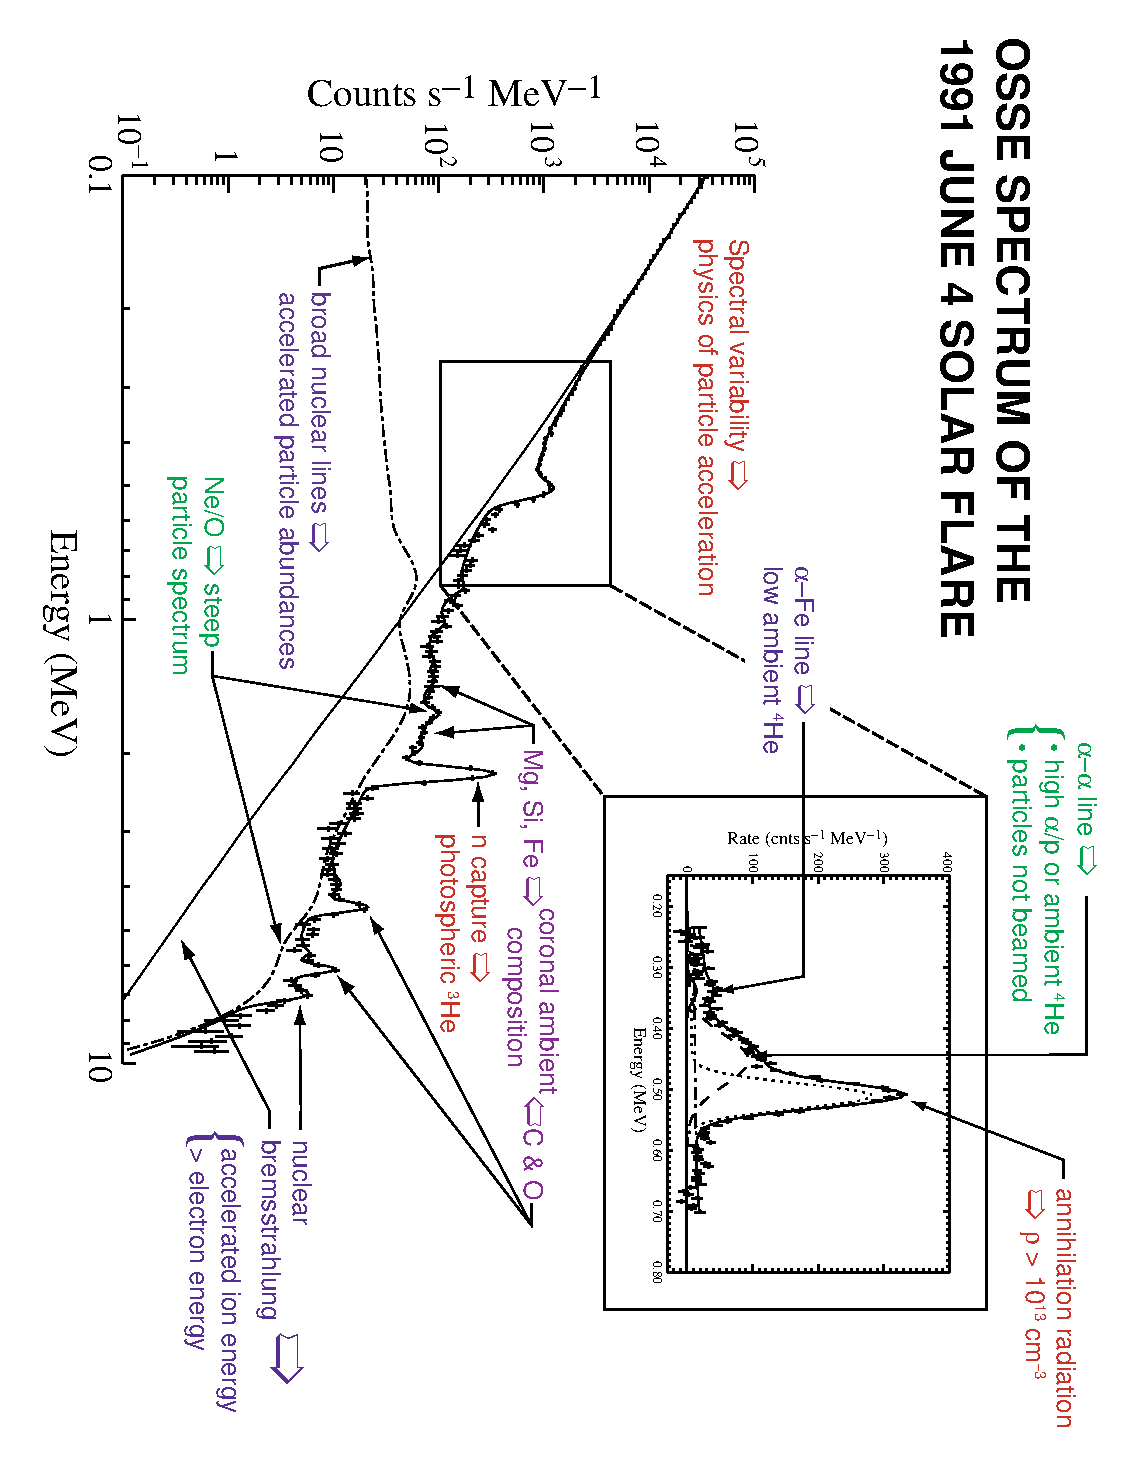
\includegraphics[width=0.75\textwidth,angle=90]{gamma-espectro.eps}
        \caption{Espectro de rayos $\gamma$ solares asociados a la explosión del \num{4} de Junio de \num{1991}. Imagen tomada de \url{https://heasarc.gsfc.nasa.gov}}
        \label{fig:gamma-espectro}
\end{figure}

A partir de la década de los noventa, observaciones en una amplio espectro (\SI{10}{\kilo\electronvolt} a \SI{30}{\giga\electronvolt}) de energías se han llevado a cabo por cuatro misiones nuevas: BASTE, OSSE, COMPTEL y EGRET. Del año \num{2000} a la fecha, dos satélites se han convertido en los principales pioneros de la observación de rayos $\gamma$: RHESSI (Reuven Ramaty High Energy Solar Spectroscopic Imager) y \emph{Fermi} (Fermi Gamma-ray Space Telescope).

El satélite RHESSI ha abierto una nueva era en las investigaciones de la aceleración de partículas en el Sol. La principal característica de este telescopio es su capacidad de producir imágenes de la atmósfera solar con una excelente resolución en un rango de energías de \SI{3}{\kilo\electronvolt} a \SI{20}{\electronvolt}. Con estas propiedades RHESSI dio la primera evidencia de sobre la localización del sitio de aceleración de los iones energéticos a través de la observación en rayos $\gamma$ \cite{hurford03,hurford06}. La figura \ref{fig:flare-foot} muestra los \emph{footprints} donde se origina la aceleración de iones/electrones. La imagen compuesta está montada sobre una fotografía tomada por el instrumento TRACE en la banda de \SI{19.5}{\nano\metre} (útil para observar la corona y plasma caliente). Estas observaciones demuestran que el sitio de aceleración es cercano a la región de la explosión, lo cual apuntaría a que está relacionada con el proceso de reconexión magnética. No obstante, no es posible explicar la diferencia entre la región de aceleración de los iones y electrones (del orden de \SI{10}{\mega\metre}).

\begin{figure}
        \centering
        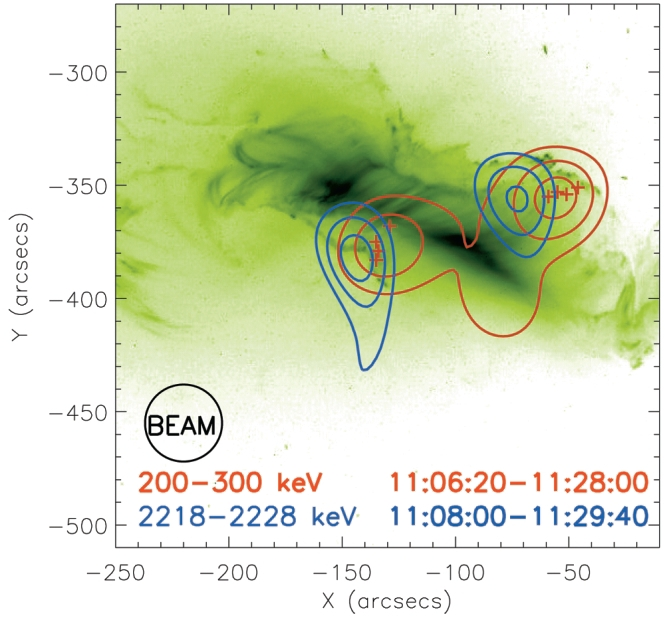
\includegraphics[width=0.75\textwidth]{flare-footprints}
        \caption{Imagen compuesta de observaciones en rayos X y $\gamma$ de la ráfaga solar ocurrida el \num{28} de Octubre de \num{2003}. Los contornos azules y rojos muestran la zona donde se aceleran la partículas (iones y electrones, respectivamente) dentro de la región activa que produjo la ráfaga. Imagen tomada de \cite{hurford03}.}
        \label{fig:flare-foot}
\end{figure}

El satélite Fermi fue lanzado en \num{2008} y cuenta con dos instrumentos: el GBM (Gamma-ray burst monitor) y el LAT (Large-area telescope). GBM es un contador de rayos $\gamma$ que se compone de dos cristales de  germanato de bismuto (\ce{BGO}) y \num{14} centelladores de yoduro de Sodio (\ce{NaI}), que en conjunto permiten analizar el espectro de radiación en un rango de \SI{8}{\kilo\electronvolt} a \SI{40}{\mega\electronvolt}. Por otro lado el instrumento LAT es un telescopio de conversión de pares y es sensible en el rango de \SI{20}{\mega\electronvolt} a \SI{300}{\giga\electronvolt}. Es importante recalcar que mientras el LAT es instrumento capaz apuntar en una cierta dirección, el GBM solo es capaz de observar incrementos en el número de partículas.

Desde su lanzamiento el instrumento LAT ha detectado tanto eventos impulsivos como eventos de larga duración, asociados con ráfagas del tipo X y M. Un descubrimiento importante dentro de estas observaciones son las emisiones de larga duración, las cuales pueden durar más de \SI{12}{\hour}, y son registradas en los rayos $\gamma$ de más alta energía ($>\SI{100}{\mega\electronvolt}$) \cite{ackermann14}. Un aspecto importante de este tipo de emisiones es que no se observan en la misma escala de tiempo en otras longitudes de onda.

En \cite{ackermann14} también se discute la posibilidad del origen de la emisión de larga duración, lo cual se hace con base en los datos del LAT asociados a una explosión ocurrida el \num{7} de Marzo de \num{2011}. En ésta se detectaron rayos $\gamma$ de hasta \SI{1}{\giga\electronvolt}, posible prueba de que fueron generados por decaimiento de $\pi^{0}$ y que la energía de los protones primarios sería del orden de \SI{5}{\giga\electronvolt}. En contraste, si la emisión es ocasionada por Bremsstrahlung de electrones energéticos, el espectro de éstos últimos debe extenderse más allá de \SI{1}{\giga\electronvolt}. Esta segunda opción resulta más compleja de empatar con otras observaciones, por lo que el decaimiento de piones parece un escenario más probable.

\section{Observación de neutrones solares}
\subsection{Propagación de neutrones solares}

Cuando los neutrones escapan de la atmósfera solar viajan sin ser afectados por los campos magnéticos en el medio interplanetario. Los neutrones libres son inestables y están sujetos a decaimiento $\beta$ con una vida media de $\tau=\SI{880.3}{\second}$. Debido a esto, el espectro de neutrones que arriban a la orbita terrestre se modifica, afectando principalmente a los neutrones de baja energía. Para tener un modelo cuantitativo de este efecto usaremos la siguiente expresión; la probabilidad de que una partícula con $\tau$ tiempo de vida media, sobreviva y alcance la Tierra sin decaer:

\begin{equation}
P\left(E_{k},r\right)=\exp\left(-\frac{t}{\gamma\tau}\right)
\end{equation}

en donde $E_{k}$ es la energía cinética de la partícula, $r$ es la distancia a la fuente (para neutrones solares $r=\SI{1}{AU}$), $t$ es el tiempo de vuelo de la partícula y $\gamma$ es factor de Lorentz. Denominaremos $P(E_{k},1AU)$ como la probabilidad de arribo de neutrones. Para neutrones con energías cinéticas $E_{k}=\SI{100}{\mega\electronvolt}$ el tiempo de vuelo es de aproximadamente \SI{1165}{\second}, con lo cual decaen el \SI{70}{\percent} de las partículas emitidas. Luego entonces, los neutrones solares con esta energía pueden ser detectados en el espacio o en superficie. Un aspecto interesante es que los productos del decaimiento (protones y electrones) también se observan, siempre y cuando se logren distinguir de la emisión de protones solares; lo cual se ha reportado con anterioridad \cite{evenson83,agueda11}.

El panel de la izquierda en la figura \ref{fig:neutron-prob} muestra la probabilidad de arribo de neutrones en el rango de energías de \num{10}-\SI{1000}{\mega\electronvolt}. La utilidad de esta gráfica viene de que puede ser utilizada como función de respuesta para corregir el espectro de energías de neutrones solares observado en el Tierra. Como se observa en la figura, en principio es posible detectar neutrones de bajas energías, sin embargo más adelante veremos que la principal limitante es la atenuación atmosférica. El panel de la derecha muestra el tiempo de vuelo en función de la energía cinética de los neutrones.

\begin{figure}
        \centering
        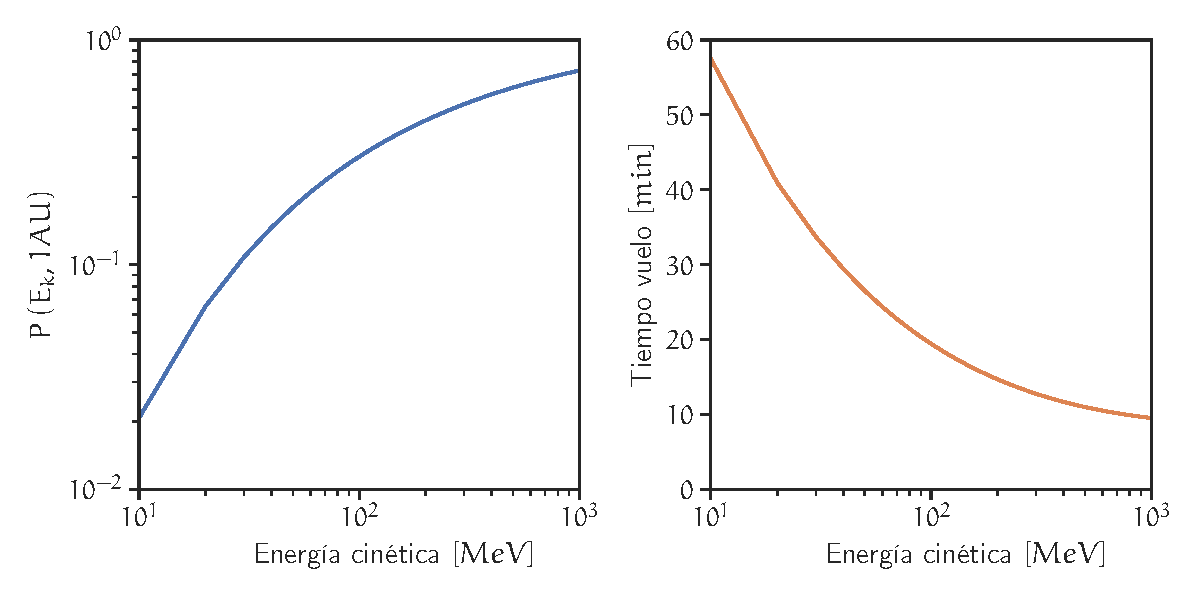
\includegraphics[width=\textwidth]{neutron-prob.pdf}
        \caption{Probabilidad de arribo de neutrones solares a la orbita terrestre (panel izquierdo) y tiempo de vuelo (panel derecho).}
        \label{fig:neutron-prob}
\end{figure}

Los neutrones que inciden al tope de la atmósfera terrestre se propagan hacia la superficie colisionando en el trayecto con núcleos atmosféricos. Durante el trayecto, tres procesos importantes ocurren: dispersión elástica, dispersión inelástica e intercambio de carga.

El proceso de dispersión elástica es el único que contribuye de manera positiva a la propagación de neutrones ya que la transferencia de energía de los neutrones a los núcleos atmosféricos es limitada en núcleos de Oxigeno y Nitrógeno (máximo $0.22$ de la energía incidente en el caso del Oxigeno y $0.28$ para el caso del Nitrógeno). Luego entonces, es de esperarse que la mayoría de los neutrones sujetos a este proceso lleguen a altitudes de alta montaña; no obstante con modificaciones en el espectro de energía y distribución angular. Los dos procesos restantes contribuyen a la atenuación de los neutrones solares. En el proceso de intercambio de carga los neutrones interaccionan con núcleos atmosféricos y en su lugar se emiten protones en la dirección frontal. En este caso la transferencia de energía es casi total y los protones emitidos son absorbidos en la atmósfera mediante ionización. Por otro lado, en la dispersión inelástica los neutrones proyectiles transfieren energía a los núcleos dejándolos en un estado excitado y generando una gran cantidad de productos secundarios (entre ellos neutrones secundarios). De manera general la dispersión inelástica contribuye de manera importante a la atenuación de los neutrones, no obstante sus productos pueden ser observados a cierta profundidad atmosférica \cite{shibata94}.

La figura \ref{fig:neutron-at} muestra el resultado de una simulación monte carlo (MC) de la propagación de \num{e8} neutrones solares en la atmósfera terrestre. Para realizar la simulación utilicé el modelo de Shibata \cite{shibata94}, el cual permite estudiar el espectro de los neutrones solares a diferentes profundidades atmosféricas y además ha sido calibrado con experimentos en aceleradores de partículas. En el modelo, los neutrones se inyectan al tope de la atmósfera con un ángulo cenital definido (para este caso $\theta=0$) y un índice espectral. Como se aprecia en la figura la mayor atenuación la sufren los neutrones de baja energía, independientemente de la profundidad, volviéndose factible detectar neutrones solares a partir de \SI{100}{\mega\electronvolt}. Por otro lado, también es posible estudiar los efectos de la atenuación en función de una profundidad especifica. De la figura se puede concluir que las localidades de alta montaña tienen características apropiadas para la observación de neutrones.

\begin{figure}
        \centering
        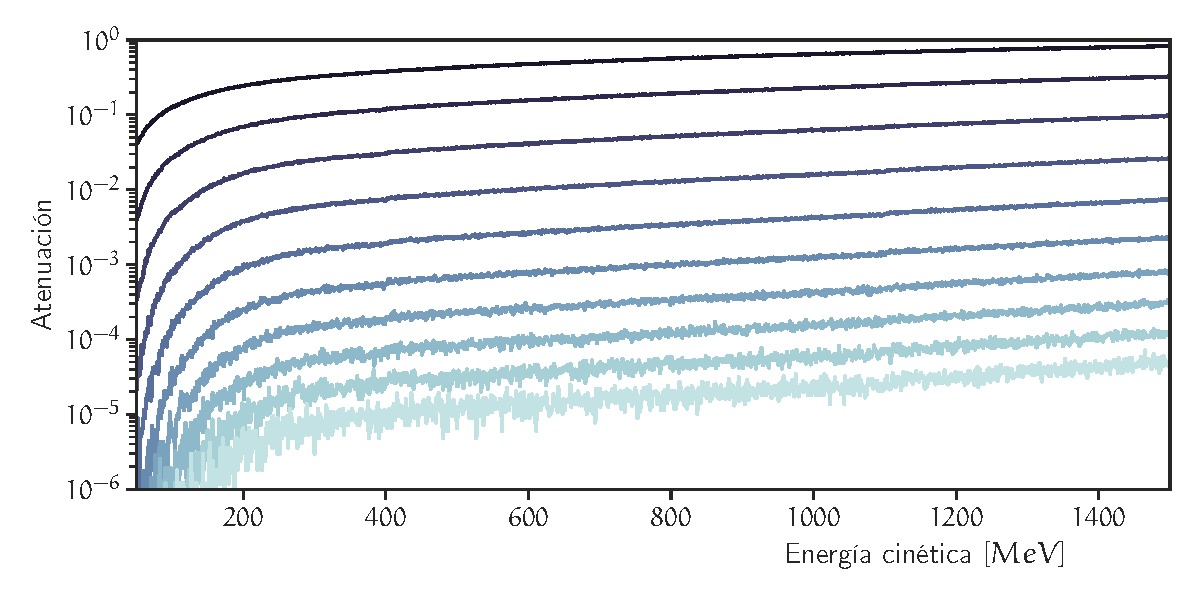
\includegraphics[width=\textwidth]{neutron-at.pdf}
        \caption{Simulación MC de la atenuación de neutrones solares en función de la energía cinética al tope de la atmósfera y profundidad atmosférica. Del color más oscuro al más claro, la profundidad atmosférica varia de \SI{100}{\gram\per\square\cm} a \SI{1000}{\gram\per\square\cm}.}
        \label{fig:neutron-at}
\end{figure}

Otra característica importante a estudiar es el perfil temporal de los neutrones cuando arriban a una cierta localidad, el cual está directamente relacionado con su espectro de energía. En la figura \ref{fig:neutron-time} muestro el resultado de simular neutrones con diferentes índices espectrales (entre \num{-3.0} y \num{-5.0}) arribando a la profundidad de Sierra Negra (\SI{575}{\gram\per\square\cm}). Como es de esperarse, al disminuir el índice espectral, los neutrones de menor energía se vuelven más dominantes en el espectro y por lo tanto, el tiempo de vuelo de los neutrones emitidos por el Sol se ve retardado. Esta propiedad de los neutrones nos permite diferenciar entre distintos mecanismos de aceleración (ver sección \ref{sec:acel-part}).

\begin{figure}
        \centering
        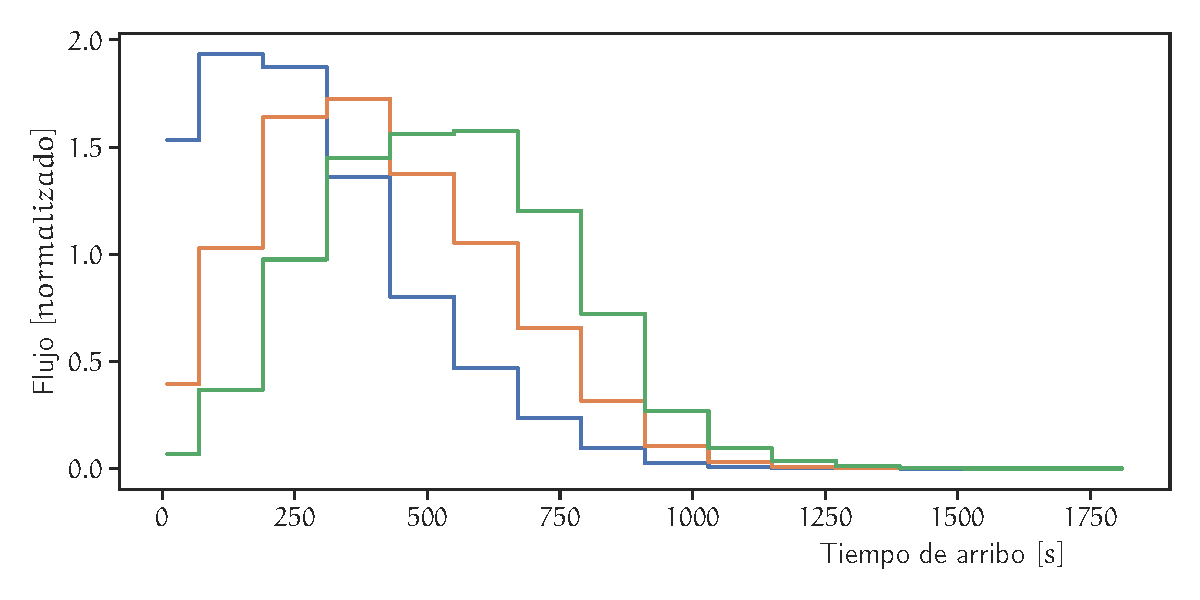
\includegraphics[width=\textwidth]{neutron-time.pdf}
        \caption{Perfiles temporales del arribo de neutrones en función del índice espectral $\alpha$. En azul $\alpha=3.0$, naranja $\alpha=4.0$ y verde $\alpha=5.0$.}
        \label{fig:neutron-time}
\end{figure}

\subsection{Observaciones en el espacio y superficie}

La primera prueba científica sobre la existencia de neutrones solares fue dada por \cite{chupp82}, en relación con la fulguración del \num{21} de Junio de \num{1980} a las \DTMtime{13:18:20} UT. El evento fue registrado por el espectrómetro de rayos $\gamma$ del satélite SMM, con un incremento total de $130\sigma$. El espectrómetro (GRS por sus siglas en inglés) está compuesto de \num{7} detectores de \ce{NaI(Tl)}, los cuales registran rayos $\gamma$ en el rango de \num{0.3} a \SI{0.9}{\mega\electronvolt}. Además el satélite cuenta con un detector de \ce{CsI(Na)} de \SI{25}{\centi\metre} de espesor, sensible a rayos $\gamma$ de alta energía y neutrones, y un sistema de anti-coincidencias.

Los datos del GRS registran tanto rayos $\gamma$ como neutrones con energías mayores a los \SI{100}{\mega\electronvolt}, lo cual brinda pruebas de aceleración de iones a energías del orden de los \si{\giga\electronvolt}. La figura \ref{fig:solar-neutrons} muestra el perfil temporal del GRS en dos bandas de deposición de energía: en panel superior de \num{10} a \SI{140}{\mega\electronvolt} y el panel inferior de \num{25} a \SI{140}{\mega\electronvolt}.

Durante la fase impulsiva de la ráfaga, que dura aproximadamente \SI{1}{\minute}, se detectaron fotones de alta energía provenientes del decaimiento de piones neutros y Bremsstrahlung de electrones. Posteriormente durante \SI{17}{\minute} se detectó el incremento debido al flujo de neutrones solares. Para la determinación del espectro de energía de los neutrones se supuso que éstos fueron emitidos con una distribución temporal $\delta$ al mismo instante que los fotones de alta energía. De acuerdo con el tiempo de vuelo registrado en los datos de la figura \ref{fig:solar-neutrons}, las energías cinéticas se extienden desde los \SI{50}{\mega\electronvolt} hasta más allá de los \SI{500}{\mega\electronvolt}. La prueba contundente de la detección de neutrones solares está en que la emisión extendida solo se registra en el canal de más alta deposición de energía y el espectro de energía no tiene la forma del espectro de fotones energéticos producidos por Bremsstrahlung \cite{dorman}.

\begin{figure}
        \centering
        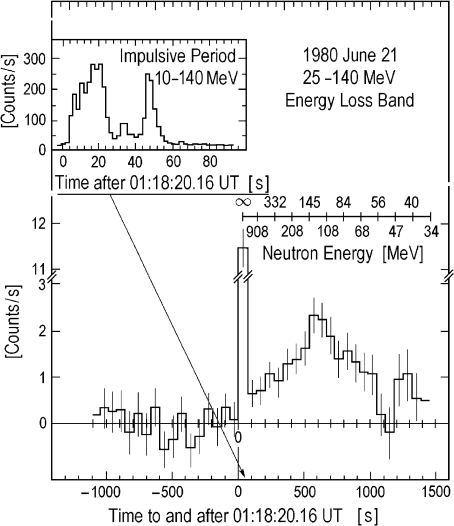
\includegraphics[width=0.6\textwidth]{solar-neutrons.png}
        \caption{Evento de neutrones solares registrado el \num{21} de Junio de \SI{1980} por el satélite SMM. El panel superior muestra el canal de menor deposición de energía y que registra el incremento debido a rayos $\gamma$. El panel central muestra los eventos con mayor deposición de energía y que corresponden a neutrones solares. Imagen tomada de \cite{chupp82}.}
        \label{fig:solar-neutrons}
\end{figure}

El \num{3} de Junio de \num{1982} se obtuvo la primera observación de neutrones solares en superficie, la cual además se observó también por medio del satélite SMM \cite{debrunner83}. El flujo de neutrones y fotones de alta energía fue originado por una intensa ráfaga X\num{8.0} que inició a las \DTMtime{11:41:00} UT. Los fotones se pudieron observar desde las ondas de radio hasta los rayos $\gamma$. A las \DTMtime{11:43:00} UT el satélite SMM registró un incremento importante en el flujo de rayos $\gamma$ provenientes del Sol, a lo que siguió una emisión de rayos $\gamma$ de alta energía ($>\SI{10}{\mega\electronvolt}$) y neutrones solares.

En la superficie terrestre \num{3} monitores de neutrones registraron incrementos sobre su nivel de fondo que van desde los $2.9$ hasta los $8.5\sigma$ \cite{chupp87}. De los tres monitores localizados en el continente Europeo el que tuvo mejores condiciones para observar el evento fue el de Jungfraujoch, Suiza\footnote{Los otros dos se localizan en Italia y la República Checa}: con un ángulo cenital solar de $\theta=\SI{25}{\degree}$ y una profundidad atmosférica de \SI{670}{\gram\per\square\cm}. La figura \ref{fig:neutrons-ground} muestra las tasas de cuentas del SMM y las del monitor de neutrones. El panel superior se encuentran los datos del GRS con una resolución de \SI{20}{\second}, mientras que el panel inferior contiene datos del NM con resolución de \SI{1}{\minute} (curva continua) y \SI{5}{\minute} (curva punteada). En los datos de \SI{5}{\minute} los incrementos de las \DTMtime{11:45:00} a \DTMtime{11:55:00} corresponden a $6.7\sigma$ y $4.0\sigma$, respectivamente. La escala de energías en el panel superior indica la energía cinética de los neutrones solares detectados, asumiendo que se emitieron al mismo instante de los rayos $\gamma$ con una distribución temporal $\delta$.

De acuerdo con \cite{chupp87} la energía de los neutrones detectados está en el rango de \SI{100}{\mega\electronvolt} a \SI{2}{\giga\electronvolt}, con un índice espectral de $-2.4$.

\begin{figure}
        \centering
        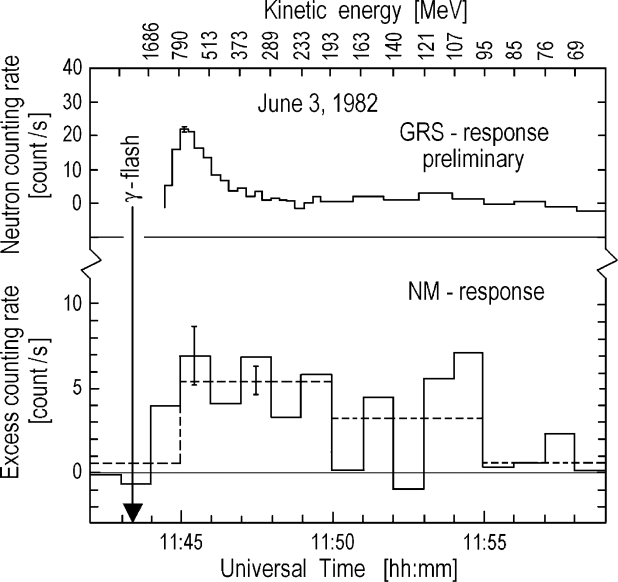
\includegraphics[width=0.5\textwidth]{neutrons-ground.png}
        \caption{Evento de neutrones solares del \num{3} de Junio de \num{1982}. El panel superior muestra los datos del SMM y el panel inferior los del monitor de neutrones de Jungfraujoch. Imagen tomada de \cite{debrunner83}.}
        \label{fig:neutrons-ground}
\end{figure}

El evento de neutrones solares del \num{22} de Febrero de \num{1991} significa un paso importante en el estudio de este fenómeno; no sólo por el estudio del evento en si, sino por la implementación exitosa del primer telescopio de neutrones solares (TNS) en el monte Norikura, Japón \cite{muraki92}. Con este nuevo instrumento fue posible discriminar la dirección de arribo de los neutrones (\SI{11}{\degree} en la dirección solar) y separarlos en bandas de energías. Las tres bandas de energías que registra el TNS son: \num{50} a \SI{360}{\mega\electronvolt}, \num{280} a \SI{500}{\mega\electronvolt} y energías mayores a \SI{390}{\mega\electronvolt}. Este evento también es de gran interés dado que la fulguración no mostró una gran significancia en la emisión de rayos X, lo cual llevo a concluir que la producción de neutrones se genero en la cromósfera baja \cite{muraki91}.

Debido al éxito del TNS de Norikura para extraer información sobre los neutrones solares, el Solar-Terrestrial Environment Laboratory (STELab) de la Universidad de Nagoya, Japón, desarrolló e instaló una red mundial de telescopios en siete montañas alrededor del mundo. La figura \ref{fig:tns-mexico} muestra un diagrama esquemático de uno de los TNS instalados en la cima del volcán Sierra Negra ($\ang{19.0}\mathbf{N}$, $\ang{97.3}\mathbf{W}$ a \SI{4580}{\metre} de altura). El telescopio está compuesto por plásticos centelladores de \SI{1}{\square\metre} de área y \SI{30}{\centi\metre} de espesor, cada uno. En total se tienen cuatro plásticos para cubrir un área de \SI{4}{\square\metre}. En los plásticos, la energía cinética de las partículas es convertida en pulsos de luz, que después son captados por un fotomultiplicador y discriminados. De esta manera, la información que registra el detector se clasifica en \num{4} canales de energía\cite{valdes04}.

\begin{figure}
        \centering
        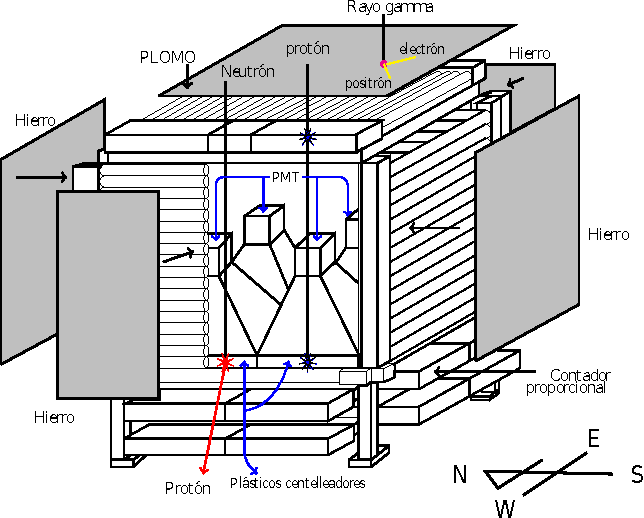
\includegraphics[width=0.7\textwidth]{tns-mexico.pdf}
        \caption{Diagrama esquemático del Telescopio de neutrones solares se encuentra en estación en la cima del volcán Sierra Negra. El sitio es conocido por albergar otro experimento importante, el Gran Telescopio Milimétrico. Las dimensiones del detector son: \SI{280}{\centi\metre} de alto y \SI{266}{\centi\metre} de largo y ancho Tomado de \cite{barrantes18}}
        \label{fig:tns-mexico}
\end{figure}

Los TNS requieren la capacidad de rechazar la componente cargada de la radiación cósmica, lo cual se logra en el caso del telescopio de Sierra Negra a través de una señal de anti-coincidencia generada por contadores proporcionales alrededor del detector. Adicionalmente, debajo del arreglo de plásticos centelladores se colocaron cuatro capas de contadores proporcionales con nueve tubos cada una, las cuales sirven para determinar la dirección de los neutrones incidentes. A pesar de sus enormes ventajas con respecto a los monitores de neutrones para observar eventos de neutrones solares, en el capítulo \ref{chap:dos} profundizaré sobre las limitantes de este diseño de telescopio.

La tabla \ref{table:eventos-neutrones} resume los eventos de neutrones solares detectados en superficie con suficiente significancia estadística ($>5\sigma$), recopilada a partir de \cite{watanabe05,sako06,muraki16}. Los eventos de la tabla han sido observados ya sea por NM, TNS o ambos. Por otra parte, una lista detallada de posibles eventos (significancias entre $2.7\sigma$ y $4.9\sigma$) de \num{1980} a \num{2005} se puede encontrar en \cite{mirosh15}.

\begin{table}
\caption{Eventos de neutrones solares detectados en superficie asociados con fulguraciones solares.}
\label{table:eventos-neutrones}

\begin{tabular}{ccccccc}
\multicolumn{7}{c}{}\\
\cmidrule(r){1-7}
Fecha & Hora & Tipo de & Localidad. & Observatorio & Índice & Flujo (\SI{100}{\mega\electronvolt})\\
 & UT & ráfaga &  &  & espectral & $\times\SI{e26}{\per\mega\electronvolt\per\steradian}$ \\
\addlinespace[5pt]
\cmidrule(r){1-7}
\num{03}/\num{06}/\num{1982} & \DTMtime{11:43:00} & X8.0 & S09E72 & Jungfraujoch & \num{-4.0(2)} & \num{260(70)}\\
\num{24}/\num{05}/\num{1990} & \DTMtime{20:48:00} & X9.3 & N36W76 & Climax & \num{-2.9(1)} & \num{430(40)}\\
\num{23}/\num{03}/\num{1991} & \DTMtime{22:42:00} & X9.4 & S26E28 & Haleakala & \num{-2.7(1)} & \num{6.0(1)}\\
\num{04}/\num{06}/\num{1991} & \DTMtime{03:37:00} & X12.0 & N30E70 & Norikura & \num{-4.9(6)} & \num{19(2)}\\
\num{24}/\num{11}/\num{2000} & \DTMtime{14:51:00} & X2.3 & N22W07 & Chacaltaya & \num{-4.2(5)} & \num{4.0(13)}\\
\num{25}/\num{08}/\num{2001} & \DTMtime{16:23:00} & X5.3 & S17E34 & Chacaltaya & \num{-3.1(4)} & \num{2.4(13)}\\
\num{28}/\num{10}/\num{2003} & \DTMtime{09:51:00} & X17.4 & S16E08 & Tsumeb & \num{-3.8(4)} & \num{37(14)}\\
\num{02}/\num{11}/\num{2003} & \DTMtime{17:03:00} & X8.3 & S14W56 & Chacaltaya & \num{-7.0(13)} & \num{2.8(16)}\\
\num{04}/\num{11}/\num{2004} & \DTMtime{19:29:00} & X28.0 & S19W83 & Haleakala & \num{-3.9(5)} & \num{150(60)}\\
\num{07}/\num{09}/\num{2005} & \DTMtime{17:17:00} & X17.0 & S06E89 & Chacaltaya & \num{-3.8} & \num{61}\\
 &  &  &  & Sierra Negra &  & \\
\num{08}/\num{07}/\num{2014} & \DTMtime{16:20:00} & M6.5 & N12E56 & Chacaltaya & \num{-2.6(2)} & \num{3.50(3)}\\
 &  &  &  & Sierra Negra &  & \\
\addlinespace[5pt]
\bottomrule

\end{tabular}
\end{table}

El evento del \num{7} de Septiembre de \num{2005} es de gran importancia debido a que ha generado una discusión importante sobre la distribución temporal de la producción de neutrones en el Sol \cite{sako06}, ya que estos son acelerados por un mayor tiempo que la radiación electromagnética. De acuerdo con \cite{watanabe09} este comportamiento puede ser explicado por un nuevo modelo de MHD desarrollado por  \cite{hua02}. En nuestro caso este evento se analizará con mayor profundidad en el capítulo \ref{chap:tres}, ya que además nos ayudará a plantear la motivación detrás del desarrollo de la nueva electrónica del SciCRT.
